\chapter{Definizione del progetto}
\setcounter{section}{1}
\item
\subsection{Architettura del progetto}
\subsubsection{Concetto Provider/Subscriber}
Il modello di \textit{provider/subscriber} definisce un flusso unidirezionale di informazioni da un oggetto \textit{provider} a un numero qualsiasi di oggetti \textit{subscribers}. Il concetto \`{e} che il \textit{provider}, anche chiamato \textit{publish}, ha informazioni o eventi utili che devono essere comunicati ad altri oggetti, ovvero tutti i suoi \textit{subscriber}, che useranno tali informazioni per eseguire azioni aggiuntive o rimanere sincronizzati con il fornitore. 

\begin{figure}[htbp]
\centering
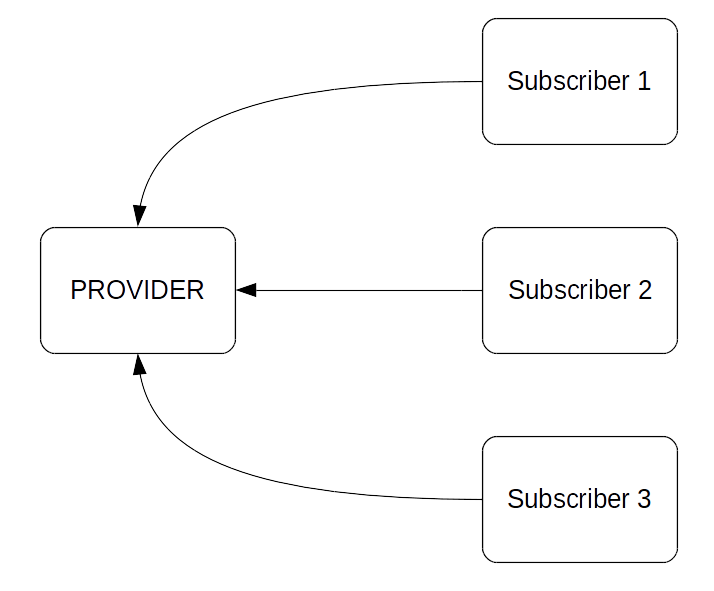
\includegraphics[scale=0.55]{img/pubsub_1.png}\\
\caption{Semplice esempio di un Provider e tre Subscriber abbonati \label{figura1.14}}
\end{figure}

Come anticipato nel capitolo precedente, la struttura base del sistema di replicazione Pglogical utilizza il modello \textit{publish/subscriber} sopra descritto.\\
Al \textit{provider} sono "abbonati" uno o pi\`{u} nodi \textit{subscribers}. Ogni nodo che riceve i dati di replica da una fonte, quindi \textit{provider}, pu\`{o} essere configurato per essere in grado di inoltrare tali dati agli altri nodi sottoscritti a s\`{e}.\\
Utilizzando la replica in cascata, ogni nodo \textit{subscriber} \`{e} in contemporanea mittente e destinatario. Pi\`{u} nello specifico, ogni sottoscrittore \`{e} anche \textit{provider} di altri \textit{subscribers}.\\ 
Ci sono tre idee distinte dietro questa capacit\`{a}:

\begin{enumerate}
\item 
La scalabilit\`{a}: un database, in particolare il \textit{publish} che riceve tutte le transazioni di aggiornamento dalle applicazioni client, ha solo una capacit\`{a} limitata di soddisfare le query dei nodi sottoscritti durante il processo di replica. 
%Per soddisfare la necessit\`{a} di un gran numero di sistemi slave di sola lettura deve essere possibile eseguire una cascata.
\item
Limitare la larghezza di banda network richiesta per un sito di backup mantenendo la possibilit\`{a} di avere pi\`{u} slave nella posizione remota.
\item
Essere in grado di configurare scenari di \textit{failover}: in una configurazione da master a slave multipli, \`{e} improbabile che tutti i nodi slave siano esattamente nello stesso stato di sincronizzazione quando il master fallisce. Per garantire che uno slave possa essere promosso al master \`{e} necessario che tutti i sistemi rimanenti possano concordare lo stato dei dati. Poich\'{e} non \`{e} possibile eseguire il \textit{rollback} di una transazione confermata, questo stato \`{e} indubbiamente lo stato di sincronizzazione pi\`{u} recente di tutti i nodi slave rimanenti.\\
\end{enumerate}

%presi da slony I - ANDRANNO BENE?
Aggiunto alle funzionalit\`{a} di PostgreSQL, che ci permette di replicare un intero database, il sistema di replicazione Pglogical pu\`{o} essere configurato per replicare in modo selettivo le righe di una tabella su entrambi i lati \textit{publisher/subscriber}.\\
Le sequenze e le tabelle sono raggruppate in modo logico dentro un set di replica (\textit{replication set}). \\
Ogni set corrisponde ai dati da replicare. \`{E} composto da una serie di flussi di dati di replica, che definiremo con $R_n$ (dove \verb"n" rappresenta la \verb"n-esimo" set di replica), contenente un gruppo di oggetti da replicare indipendenti da altri oggetti provenienti dallo stesso master. In ogni caso, tutte le tabelle che hanno relazioni che potrebbero essere espresse come vincoli di chiavi esterne e tutte le sequenze utilizzate per generare numeri di serie in queste tabelle dovrebbero essere contenute in uno stesso set.

\begin{center}
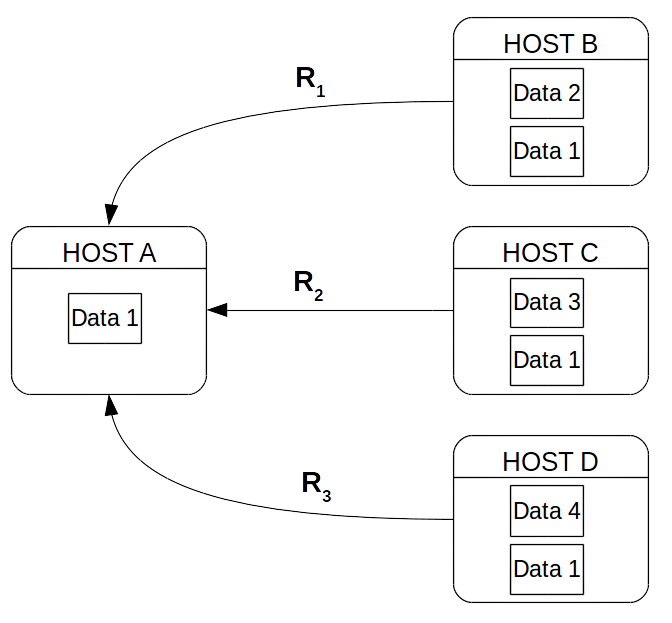
\includegraphics[scale=0.60]{img/setreplica.png}
\end{center}
\begin{figure}[htbp]
\caption{Set di replica o (\textit{replication set}) \label{figura1.15}}
\end{figure}

%I parametri sono principalmente per server di invio e standby, sebbene alcuni parametri abbiano significato solo sul server master. Le impostazioni possono variare nel cluster senza problemi se necessario.
La figura illustra un semplice esempio di una configurazione di replica. Il set di replica \`{e} composto dal flusso di dati $R_1$, $R_2$ e $R_3$.
Questo scenario raffigura quattro host (nel seguente caso quattro nodi) in cui il \textbf{NODO A} ha il ruolo di \textit{publish} e i restanti sono i suoi sottoscrittori.\\
\verb"Data 1" rappresenta il flusso di dati nativi di \textbf{A} da replicare. Ciascun \textit{subscriber}, in aggiunta ai propri nativi (\verb"Data 2", \verb"Data 3" e \verb"Data 4"), ha esattamente i dati originali del \textbf{NODO A}, in quanto abbonati. \\
In questo modo se fallisce una scrittura di nuovi dati sul \textit{provider}, l'\textbf{HOST B}, in quanto suo successivo, pu\`{o} essere promosso come \textit{master} della sottoscrizione di replica.
\subsection{Simulazione di un filesystem distribuito (Dati e Metadati)}
Ogni file viene inserito dentro un \textit{bucket}, che \`{e} un insieme di record all'interno di un database, ovvero un oggetto, contenente un insieme di campi o elementi, ciascuno dei quali \`{e} identificato da un nome univoco e da un tipo di dato.\\
Di ciascun file vengono scritte due informazioni:
\begin{enumerate}
\item 
file intero diviso in chunk,
\item
una parte di metadato.\\
\end{enumerate}
\`{E} necessario replicare i dati/metadati sulle varie \textit{board} in modo tale che, in casi di \textit{fault}, guasti o perdite, sia possibile ottenere nuovamente il dato originale.\\
Ci domandiamo quindi: in che modo possiamo ottenere maggiore affidabilit\`{a}?
%Per i metadati la replica segue il concetto del modello \textit{provider/subscriber}. 
Quando \`{e} scritto un file, per ogni \textit{chunk} e per ogni metadato, viene generato un numero pseudocasuale che definisce un ID. 
Ogni \textit{board} gestisce un range di ID.
L'ID ottenuto \`{e} passato a una mappa che restituisce la posizione della \textit{board} a cui appartiene; pi\`{u} precisamente il suo indirizzo IP. Di conseguenza sono identificate anche le \textit{board} precedenti e successive a essa.\\
Per ottenere una garanzia della replica del dato, \`{e} indispensabile replicarlo almeno due volte su \textit{board} differenti. Il dato deve essere quindi scritto sulla \textit{board} a cui appartiene e sul suo successore.
Inizialmente una stessa \textit{board} gestiva due range diversi tra loro. Ciascuna \textit{board} conteneva perci\`{o} due nodi e quindi due database.\\
Prendiamo come esempio la \verb"BOARD 01", che per semplificare chiameremo \verb"B 01 01", dove il primo numero rappresenta lo \textit{chassis} e il secondo identifica la \textit{board}.\\
La rappresentazione della mappa avr\`{a} una forma simile a quella che segue:\\
\begin{center}
\begin{tabular}{ | l | c | r}
\hline
\textbf{BOARD} & \textbf{range ID}\\
\hline
\verb"B 01 01" & \verb"0-10"\\
\verb"B 01 02" & \verb"11-20"\\
\verb"B 01 03" & \verb"21-30"\\
\verb"B 01 01" & \verb"31-40"\\
\verb"B 01 02" & \verb"41-50"\\
\verb"B 01 03" & \verb"51-60"\\
\hline

\end{tabular}
\end{center}
\\

Da questo scenario emerge che la \verb"BOARD 01" gestisce gli ID compresi tra \verb"0-10" e \verb"51-60".\\
Il problema sta nel fatto che se la \verb"BOARD 01" muore, il successivo e quindi il \textit{subscriber}, sar\`{a} in entrambi i casi la \verb"BOARD 02".\\
Ci\`{o} \`{e} fonte di debolezza; \`{e} fondamentale che i dati siano replicati su \textit{board} diverse. Questo implica che ogni nodo di una \textit{board} deve avere nella mappa differenti successori, allo scopo di garantire una distribuzione dei dati pi\`{u} uniforme.\\
La gestione delle repliche \`{e} coordinata direttamente da PostgreSQL.
Quest ultimo consente la creazione e manipolazione efficiente di database, tuttavia ha la limitazione di replicare in modo totale i dati presenti in un host; altro motivo per cui non \`{e} possibile avere una struttura come quella raffigurata precedentemente.\\
La soluzione \`{e} fornita da Pglogical, che permette la replica selettiva di righe o tabelle, rendendo in questo modo agevole la copia su pi\`{u} \textit{board}: una riga di una tabella pu\`{o} essere replicata sulla \verb"BOARD 02" e un'altra su una diversa \textit{board}.\\
Nello scenario descritto precedentemente, in cui sono configurate due nodi per \textit{board}, contemporaneamente posso avere due connessioni (ossia due client differenti eseguono due transazioni parallele in simultanea), che richiedono la scrittura su due tabelle della stessa \textit{board}. Ad esempio: due client vogliono scrivere un dato con ID \verb"8" e \verb"58" con due transazioni parallele; i client si aspettano una risposta di successo una volta avvenuta la scrittura sulla \verb"BOARD 01" e sulla sua successiva (configurabile dal parametro \verb"synchronous_commit" di PostgreSQL). Questo non \`{e} possibile, poich\`{e} Postgres, come detto, replica un intero database.
L'occupazione del disco dei metadati rispetto a quello dei dati \`{e} decisamente minore, infatti il grosso dell'occupazione del disco sono i \textit{chunk} del file. Di fatto i metadati hanno grandezza fissa; l'unico metadato che cresce \`{e} la lista di un file presente in un \textit{bucket}. I metadati possono cambiare a runtime: c'\`{e} la necessit\`{a} di gestire la replica tramite Pglogical.
I dati, invece, quando sono scritti non cambiano nel corso del tempo, poich\`{e} hanno dimensione fissa. \\
Per questo motivo \`{e} stata fatta la seguente distinzione:

\begin{itemize}
\item 
la mappa che coordina i \textit{chunk} di un file, quindi i dati, gestisce pi\`{u} nodi per \textit{board},
\item
la mappa dei metadati, gestisce un solo nodo per \textit{board}, un solo database, quindi una sola replica (sincrona).
\end{itemize}

Siamo arrivati alla conclusione che i database per i dati e i metadati devono essere separati.\\
Ogni \textit{board} ha otto database di dati, che corrispondono a otto nodi, e uno solo di metadati.\\
Scrivere la ridondanza dei dati \`{e} di conseguenza pi\`{u} semplice: 

\begin{enumerate}
\item
viene calcolato l'ID del \textit{chunk} e il rispettivo contenuto;
\item
una funzione, a cui viene passato l'ID ottenuto, restituisce dalla mappa la \textit{board} con il range di cui fa parte e il successivo host. Nel caso in cui una \textit{board} \`{e} morta, c'\`{e} un meccanismo per cui viene restituita quella successiva ancora (fino ad arrivare a un massimo di \verb"5" \textit{board}, che corrisponde alla massima catena di replica); 
\item 
sono aperte due connessioni;
\item
il \textit{frontend} si connette a due Postgres, lanciando una query in parallelo, che permette la scrittura dei \textit{chunk} su due host differenti;
\item
sono chiuse le connessioni.
\end{enumerate}

\textbf{figura con due host e query in parallelo}
Se tutte le \textit{board} sono morte, non si effettua alcuna scrittura. Di fatto se quattro \textit{board} sono gi\`{u} ho solo una \textit{board} per scrivere il dato, non rispettando la necessit\`{a} di replicarlo almeno due volte.\\
Tuttavia la probabilit\`{a} di avere quattro \textit{board} consecutive morte \`{e} decisamente bassa.\\

Di conseguenza le repliche sono utilizzate solo per quanto riguarda i metadati. \\
Se la \verb"BOARD 01" \`{e} offline per un periodo di tempo, i metadati che devono essere replicati, sono scritti sugli host successivi; il primo \textit{subscriber} della \verb"BOARD 01" diventa appunto \textit{provider} di quel set di replica. Quando torna online la \verb"BOARD 01" non \`{e} aggiornata con gli ultimi dati replicati.\\
Sarebbe utile un meccanismo di versionamento; tuttavia \`{e} troppo complesso. \\
La replica selettiva di Pglogical consente la giusta soluzione. In questo modo la replica \`{e} coordinata direttamente da PostgreSQL. Il \textit{frontend} si connette a un host, dopodich\`{e} \`{e} il database che si replica con le funzionalit\`{a} offerte da Postgres.\\
%2a01:84a0:1001:a001::1:4;3000000000000000000000000000000000000000;4000000000000000000000000000000000000000;30000000
%2a01:84a0:1001:a001::1:5;4000000000000000000000000000000000000000;5000000000000000000000000000000000000000;40000000
%2a01:84a0:1001:a001::1:6;5000000000000000000000000000000000000000;6000000000000000000000000000000000000000;50000000
%2a01:84a0:1001:a001::2:1;6000000000000000000000000000000000000000;7000000000000000000000000000000000000000;60000000
Segue un esempio di come un metadato \`{e} rappresentato nella mappa:

%\footnotesize
\begin{center}
\verb"2a01:84a0:1001:a001::2:2;70;80;70"
\end{center}

\begin{itemize}
\item 
\verb"2a01:84a0:1001:a001" indentifica la posizione del host, quindi l'indirizzo IP della \textit{board};
\item 
la \textit{board} \`{e} la \verb"2:2" (\verb"B 02 02"): \textit{chassis} \verb"02" e board \verb"02";
\item
\verb"70;80" \`{e} il range gestito dal host individuato;
\item
l'ultimo numero, \verb"70", rappresenta il nome identificativo del database.
\end{itemize}

Consegue la rappresentazione del host preso in considerazione:

\begin{figure}[htbp]
\centering
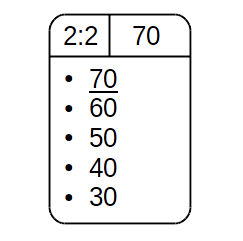
\includegraphics[scale=0.70]{img/focus_provider.png}\\
\caption{\verb"BOARD 02 02": \verb"2a01:84a0:1001:a001::2:2;70;80;70". \label{figura1.16}}
\end{figure}

Prendiamo in considerazione le \textit{board} successive all'host appena visto:

\begin{center}
\verb"2a01:84a0:1001:a001::2:2;70;80;70"
\verb"2a01:84a0:1001:a001::2:3;80;90;80"
\verb"2a01:84a0:1001:a001::2:4;90;a0;90"
\verb"2a01:84a0:1001:a001::2:5;a0;b0;a0"
\verb"2a01:84a0:1001:a001::2:6;b0;c0;b0"
\end{center}

La \verb"BOARD 02 02" \`{e} \textit{provider} dei suoi quattro host successivi (di conseguenza anche i predecessori, che non sono presenti in questa mappa d'esempio). \\
Illustriamo il set di replicazione sottoscritta:

\begin{center}
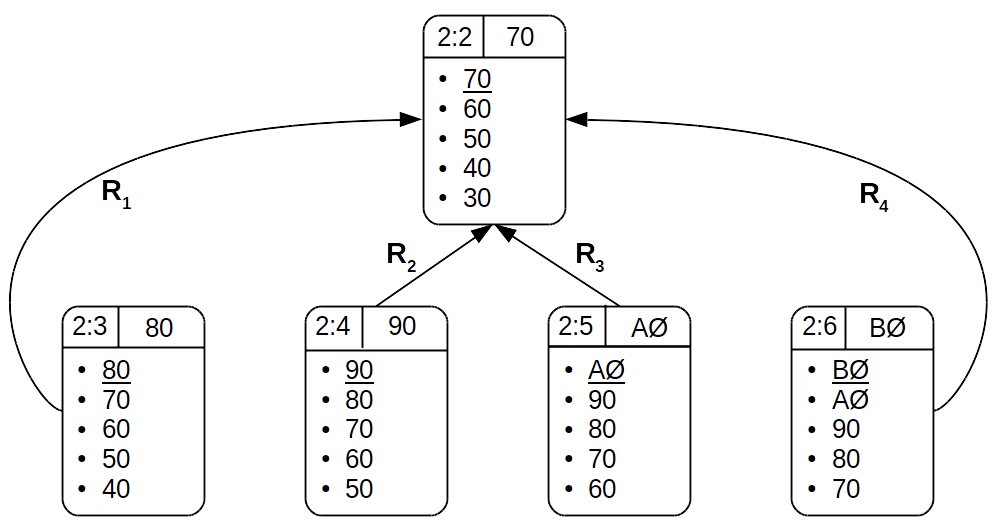
\includegraphics[scale=0.50]{img/prov_replica.png}
\end{center}
\begin{figure}[htbp]
\caption{Set di replica della \verb"BOARD 02 02" visto come \textit{provider}. \label{figura1.17}}
\end{figure}

\`{E} stato configurato che il metadato viene replicato su quattro host differenti sottoscritti alla \verb"BOARD 02".\\
$R_1$ replica i metadati con ID \verb"70, 60, 50, 40", $R_2$ \verb"70,60,50", $R_3$ \verb"70,60" e $R_4$ \verb"70".\\
A sua volta, l'host preso in considerazione, funziona come \textit{subscriber} a un altro set di replica; come segue:

\begin{center}
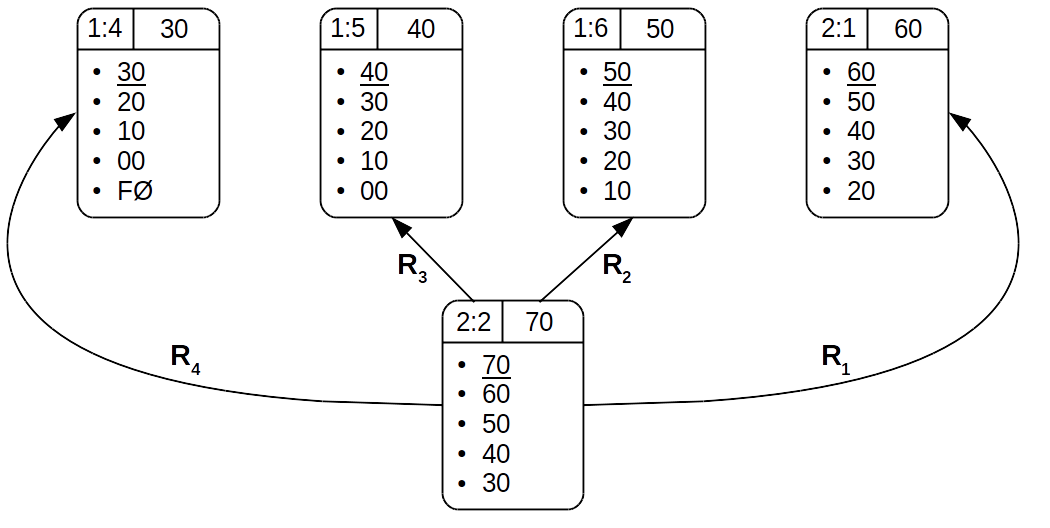
\includegraphics[scale=0.50]{img/sub_replica.png}
\end{center}
\begin{figure}[htbp]
\caption{Set di replica della \verb"BOARD 02 02" visto come \textit{subscriber}. \label{figura1.17}}
\end{figure}

In questo modo abbiamo la certezza che il metadato sia replicato su tutti i nodi (quindi su tutte le \textit{board}) a lui "abbonate". In contemporanea ogni database funge da \textit{subscriber} di altri nodi.

\subsubsection{Native subscribtions}
Fino a questo punto \`{e} stato descritto come funzionano le repliche.\\
Consideriamo il caso in cui la \verb"BOARD 02 02" sia offline per un periodo di tempo. Se il client prova a connettersi al database della \verb"BOARD 02" per scrivere un metadato che appartiene al range \verb"70-80", vede che la \textit{board} non risponde. Il metadato viene quindi scritto sulla \textit{board} immediatamente successiva alla \verb"02" nella mappa; di fatto la \verb"B 02 03" diventa il nuovo \textit{master} e il metadato viene replicato quattro volte, invece di cinque.\\
A un certo punto la \verb"BOARD 02" torna disponibile, di conseguenza tutti i metadati che appartengono a quel range possono essere scritti normalmente e replicati come illustrato nella \textit{figura 1.17}. Questo avviene per\`{o} solo nel caso in cui la \textit{board} \`{e} aggiornata.\\
Il problema sta nel fatto che non \`{e} certo che l'host \verb"02" sia sincronizzato correttamente con gli altri nodi, poich\`{e} gli eventuali nuovi metadati scritti si trovano nel database della \verb"BOARD 03".\\
Pglogical permette di gestire le repliche tra un nodo \textit{master} e una serie di \textit{slaves}. Nel nostro caso, \`{e} configurato per coordinare tanti nodi \textit{master}. \\
Per renderlo \textit{multi-master} sono state realizzate le repliche native ( \textit{native subscriptions}) che hanno direzione opposta alle repliche appena descritte.\\
Quando la \verb"BOARD 02" diventa nuovamente online, pu\`{o} ottenere i nuovi metadati scritti sul nodo successivo attraverso una fase di sincronizzazione.

\begin{center}
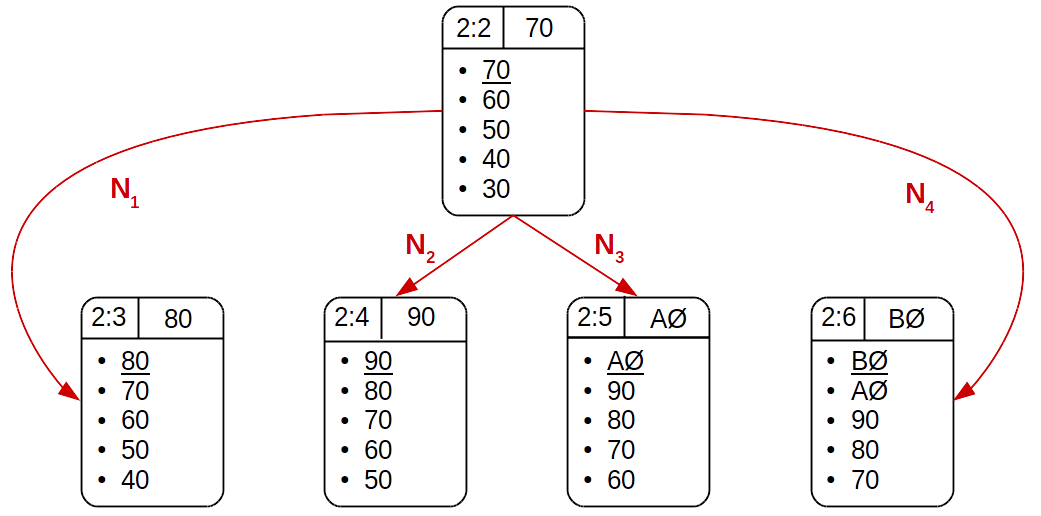
\includegraphics[scale=0.50]{img/prov_native.png}
\end{center}
\begin{figure}[htbp]
\caption{\textit{Native subscriptions} della \verb"BOARD 02 02" visto come \textit{provider}. \label{figura1.17}}
\end{figure}

Di conseguenza:

\begin{center}
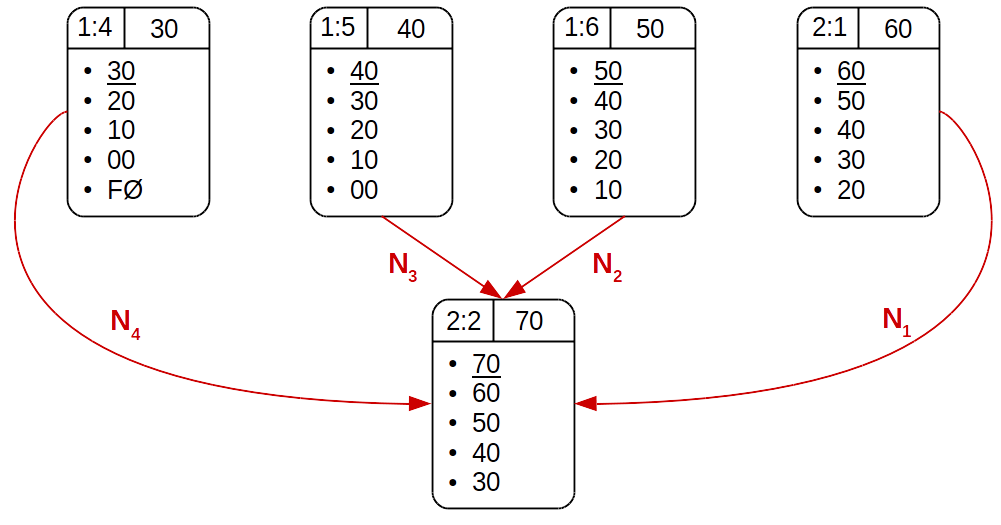
\includegraphics[scale=0.50]{img/sub_native.png}
\end{center}
\begin{figure}[htbp]
\caption{\textit{Native subscriptions} della \verb"BOARD 02 02" visto come \textit{subscriber}. \label{figura1.17}}
\end{figure}

\subsubsection{Replica sincrona e asincrona}
Quando la scrittura di un dato \`{e} andata a buon fine, viene confermata al client con un messaggio di risposta di successo. Come abbiamo detto, per una questione di affidabilit\`{a}, deve essere garantita la replicazione di un dato almeno due volte. Ci\`{o} \`{e} permesso da un importante funzionalit\`{a} di Postgres: il \verb"synchronous_commit".\\
Ci sono due tecniche di repliche che esamineremo: 
\begin{itemize}
\item 
replica asincrona 
\item
replica sincrona
\end{itemize}

La replica asincrona \`{e} un approccio \textit{store and forward}.
\`{E} la modalit\`{a} di archiviazione dei dati in cui i dati non vengono immediatamente sottoposti a backup; di fatto non aspetta che lo storage primario confermi la completa scrittura del dato sul disco. La replica asincrona ha come obiettivo di eseguire la copia di un dato in un determinato periodo di tempo prestabilito. Pi\`{u} precisamente, il client ha la conferma di avvenuto successo quando il dato da replicare \`{e} stato scritto sul WAL. Questo metodo si traduce in un sistema con buone prestazioni e minori requisiti di larghezza di banda, poich\'{e} i dati non vengono replicati in backup in tempo reale. Ci\`{o} non garantisce per\`{o} che il dato sia immediatamente disponibile, di conseguenza, questo tipo di approccio dovrebbe essere usato per dati o informazioni meno sensibili che hanno tolleranza alla perdita. Nel caso in cui, in una minima frazione di tempo, muore una \textit{board}, il dato \`{e} tracciabile solo sul WAL. La sua latenza di rete e la tolleranza della larghezza di banda lo rendono adatto per la replica a lunga distanza.\\
La replica sincrona viene utilizzata principalmente per le applicazioni transazionali di fascia alta che richiedono il \textit{failover} istantaneo in caso di guasto del nodo primario. 
Questa tecnica \`{e} preferibile per le applicazioni con obiettivi a basso tempo di recupero che non possono tollerare la perdita di dati.\\
Il seguente approccio ha i suoi svantaggi. La replica sincrona \`{e} pi\`{u} costosa di altre forme di replica dei dati, introduce la latenza che rallenta l'applicazione principale e funziona solo a brevi distanze. Il vantaggio risiede nel fatto che garantisce la scrittura della replica su un'altra \textit{board}, comunicando al client che la copia \`{e} avvenuta con successo. \\

La differenza principale tra la replica sincrona e la replica asincrona \`{e} il modo in cui i dati vengono scritti nella replica. La maggior parte dei prodotti di replica sincrona scrive i dati nello storage primario e nella replica contemporaneamente. In quanto tale, la copia primaria e la replica dovrebbero rimanere sempre sincronizzati.\\
Al contrario, i prodotti di replica asincrona scrivono prima i dati nella memoria primaria e quindi copiano i dati nella replica. Sebbene il processo di replica possa verificarsi quasi in tempo reale, \`{e} pi\`{u} comune che la replica si verifichi su base pianificata. \\
Il nostro scopo \`{e} di trovare un giusto compromesso tra garanzia e velocit\`{a} della replicazione di dati.


\subsubsection{Parametri del file di configurazione di PostgreSQL}
Analizzeremo ora i parametri che possono essere impostati sul \textit{master} che deve inviare i dati di replica ai suoi \textit{slaves} "abbonati".\\

La replica del metadato su almeno due \textit{board} \`{e} realizzabile utilizzando l'attendibilit\`{a} della tecnica di replica sincrona, ottenuta tramite PostgreSQL, con la configurazione del parametro \verb"synchronous_commit".\\
\`{E} uno dei parametri pi\`{u} importanti con una quantit\`{a} di opzioni sopra la media. Specifica se il \verb"commit" della transazione attende che i record WAL vengano scritti sul disco prima che il comando restituisca un'indicazione "riuscita" al client. 

I valori validi sono \verb"on", \verb"remote_write", \verb"local" e \verb"off". Quando una \textit{board} \`{e} \textit{offline}, pu\`{o} verificarsi un ritardo tra il momento in cui viene segnalato il successo al client e quando la transazione \`{e} realmente garantita per essere sicura contro un arresto anomalo del server. 
%(il ritardo massimo è tre volte wal_writer_delay.) 

L'impostazione di questo parametro su \verb"off" non crea alcun rischio di incoerenza del database: un sistema operativo o un arresto anomalo del database potrebbe causare la perdita di alcune transazioni presunte recenti. Pertanto, disattivare \verb"synchronous_commit" pu\`{o} essere un'alternativa utile quando le prestazioni sono pi\`{u} importanti della certezza esatta sulla durata di una transazione.\cite{etichetta12}
Nel nostro caso il \verb"synchronous_commit" \`{e} impostato a \verb"on". Ci\`{o} garantisce che il \verb"commit" delle transazioni attenda sempre che i dati vengano realmente scaricati nel log delle transazioni (ovvero nel WAL) assicurandosi che la transazione sia realmente persistente. Pi\`{u} nello specifico, ci\`{o} garantisce che la transazione non vada persa a meno che sia il \textit{master} che lo \textit{slave} subiscano un danneggiamento della memoria del database. 
Nella modalit\`{a} di replica dello streaming sincrono anche la replica deve fare lo stesso.\\

Il \verb"synchronous_standby_names" specifica l'elenco delle sottoscrizioni di replica che sono in grado di supportare la replica sincrona. \`{E} stato impostato come segue:

\begin{center}

\verb"synchronous_standby_names = '1 (r1, r2, r3, r4)'"

\end{center}

In qualsiasi momento ci sar\`{a} una replica sincrona; le transazioni in attesa di \verb"commit" saranno autorizzate a procedere dopo che questo server di standby confermer\`{a} il ricevimento dei loro dati. 
Lo \textit{standby} sincrono \`{e} il primo nominato in questo elenco. Altri server di \textit{standby} che appaiono in seguito rappresentano le potenziali repliche sincrone; nel caso in cui \verb"r1" non possa permettere la replica, disconnettendosi per qualsiasi motivo, verr\`{a} sostituito con il successivo \textit{standby} presente in questo elenco, che diventer\`{a} la nuova replica sincrona. \\

Impostare una sola replica sincrona pu\`{o} essere il giusto compromesso tra affidabilit\`{a} e velocit\`{a} di prestazioni. Il metadato, infatti, sar\`{a} copiato sicuramente due volte su host differenti: quello nativo e un sicuramente un suo \textit{subscriber} tramite la replica sincrona.\\

Questi parametri possono essere impostati solo nel file di configurazione di PostgreSQL \verb"postgresql.conf".

\section{Considerazioni statistiche sulla ridondanza sul dato}
L'occupazione dei dati del disco \`{e} maggiore rispetto a quella dei metadati, in quanto un dato rappresenta il contenuto del file stesso.\\

Durante l'\textit{upload} il file viene suddiviso in \textit{chunk} di varie dimensioni. Ogni \textit{chunk} \`{e} ridondato due volte su due diversi host.\\
Oltre la ridondanza, tramite lo \verb"XOR" byte a byte di sei \textit{chunk} viene costruito un \textit{chunk} chiamato di parit\`{a}, ridondato anch'esso due volte. 
Nel caso sia perso un \textit{chunk} appartenente al set di parit\`{a} \`{e} possibile ricostruirlo tramite il \textit{chunk} di parit\`{a}, eseguendo l'operazione inversa.

L'utilizzo di algoritmi di parit\`{a} sono applicati solo a file di svariati \textit{chunk}. Di fatto se \`{e} caricato un file di solo un \textit{chunk} di grandezza \verb"d", l'occupazione sar\`{a} \verb"4 \cdot d". Se il file \`{e} di \verb"6" \textit{chunk} l'occupazione \`{e} di \verb"14d", di cui \verb"6 \cdot 2 \cdot d" sono ottenuti dalla ridondanza dei \verb"6" \textit{chunk} e \verb"2 \cdot d" dalla ridondanza di parit\`{a}.\\
\`{E} sconveniente di conseguenza usare questo metodo di parit\`{a} per file di solo un \textit{chunk}, poich\`{e} il rapporto tra dati uploadati e dati salvati \`{e} di \verb"4" rispetto al rapporto di \verb"2,3" nel caso di file di \verb"chunk".\\

Ciascun chunk \`{e} ridondato su dischi differenti. \\
Per causare la perdita di un dato, quanti dischi possono essere danneggiati?\\

La seguente figura illustra il caso in cui \`{e} perso un chunk, quindi anche la sua ridondanza. Questo scenario garantisce tuttavia la possibilit\`{a} di ricostruire il dato, mantendo di conseguenza la sua sicurezza:

\begin{center}
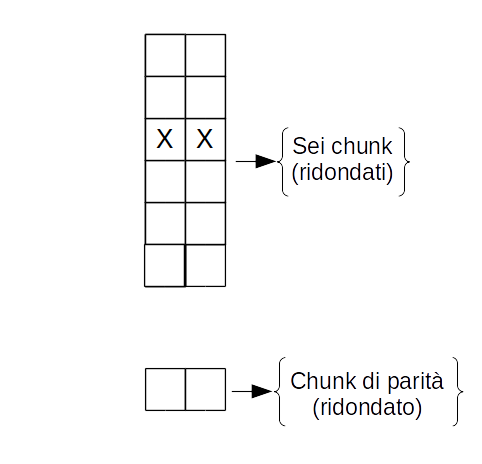
\includegraphics[scale=0.55]{img/chunk1.png}
\end{center}
\begin{figure}[htbp]
\caption{Perdita di un \textit{chunk} \label{figura1.17}}
\end{figure}

Seguono i due scenari in cui pu\`{o} accadere che un dato non possa essere recuperato.
Se viene perso un \textit{chunk} e il \textit{chunk} di parit\`{a} (quindi la sua ridondanza) non \`{e} realizzabile ricreare il dato (figura ~\ref{figura1.29}). Ugualmente se sono persi due \textit{chunk} del set di parit\`{a} (figura ~\ref{figura1.30}).

\begin{center}
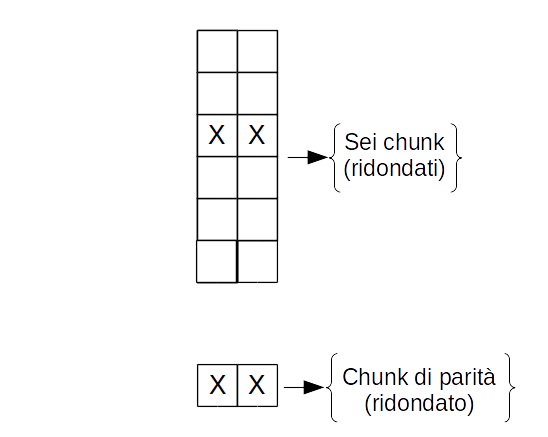
\includegraphics[scale=0.55]{img/chunk2.png}
\end{center}
\begin{figure}[htbp]
\caption{Perdita di un \textit{chunk} e del \textit{chunk} di parit\`{a} \label{figura1.29}}
\end{figure}

\begin{center}
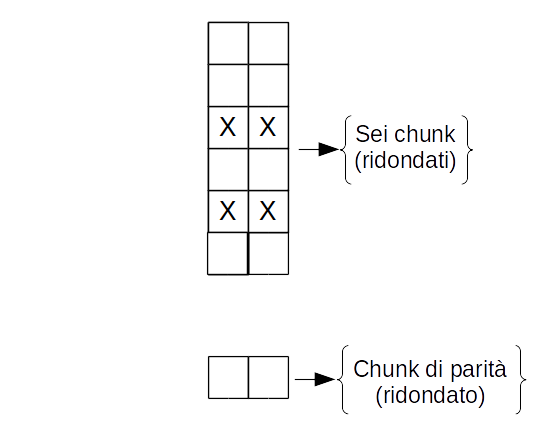
\includegraphics[scale=0.55]{img/chunk3.png}
\end{center}
\begin{figure}[htbp]
\caption{Perdita di due \textit{chunk} \label{figura1.30}}
\end{figure}

Nel peggiore dei casi la perdita di \verb"4" dischi causa l'impossibilit\`{a} di ricostruire un dato.
La probabilit\`{a} che si rompano \verb"4" dischi su \verb"228" \`{e}:

\begin{center}
\Large
\tfrac{1}{228} \cdot  \tfrac{1}{227} \cdot \tfrac{1}{226} \cdot \tfrac{1}{225}\\
\end{center}
\normalsize

Tuttavia ancora non corrisponde al caso peggiore. Questo calcolo non tiene conto che i dischi si guastano con una probabilit\`{a} di un certo tipo; solitamente i dischi si rompono con probabilit\`{a} uniforme del \verb"2%".\\

Affinch\`{e} questo accada \`{e} necessario considerare il seguente evento distribuito nel tempo.

Ad esempio consideriamo che in un anno si rompono \verb"2" dischi su \verb"100".
Se viene valutato un giorno ottengo:

\begin{center}
\Large
\tfrac{100}{365} \cdot \normalsize \verb"0,02"\\
\end{center}

che corrisponde alla probabilit\`{a} che mi si rompa il disco quel preciso giorno.\\
Consideriamo un target di \verb"3" ore per ricostruire il dato; calcoliamo la probabilit\`{a} che un disco si rompa in queste tre ore:

\begin{center}
\Large
\tfrac{\tfrac{100}{365} \cdot \normalsize \verb"0,02}{\normalsize \verb"24} \cdot \normalsize \verb"3"\\
\end{center}

Se il disco si rompesse dopo le \verb"3" ore considerate, il dato verrebbe ricostruito quindi la catena di probabilit\`{a} che rappresenta la rottura di \verb"4" dischi si annullerebbe.
Affinch\`{e} ci sia la perdita di un dato deve verificarsi la rottura di \verb"4" dischi in \verb"3" ore.\\

Fissato un tempo, nel nostro caso un giorno, la probabilit\`{a} che si danneggino tutti e quattro i dischi \`{e}:

\begin{center}
\Large
\tfrac{1}{228} \cdot  \tfrac{1}{227} \cdot \tfrac{1}{226} \cdot \tfrac{1}{225} \cdot \tfrac{\tfrac{100}{365} \cdot \normalsize \verb"0,02}{\normalsize \verb"24} \cdot \normalsize \verb"3"\\\\
\end{center}
\normalsize

La probabilit\`{a} che non si possa ricostruire un chunk in tre ore \`{e} quindi un numero veramente basso.\\

Un danneggiamento di un file avviene anche quando \`{e} perso anche solo un chunk. La probabilit\`{a} congiunta che tutti i file siano presenti e non siano andati persi rappresenta la probabilit\`{a} di avere tutto il file integro.\\
Questo varia sui file di piccole dimensioni e sui file di maggiori grandezza \`{e} una probabilit\`{a} pi\`{u} bassa.\\

La considerazione \`{e} stata fatta nel caso peggiore. In realt\`{a} la probabilit\`{a} \`{e} ulteriormente pi\`{u} bassa, in quanto ci sono altre probabilit\`{a} sfavorevoli che hanno a loro volta probabilit\`{a} maggiore.\\
La perdita di un dato \`{e} di conseguenza realmente difficile.


\section{Considerazioni statistiche sulla ridondanza sul metadato}
Il metadato \`{e} di piccole dimensioni, poich\`{e} rappresenta l'informazione anagrafica del dato. 
Per questo motivo non \`{e} conveniente utilizzare metodi di parit\`{a} per ricostruire l'informazione anche se \`{e} perso in parte.
Per il metadato \`{e} sufficiente creare quattro repliche, garantendo ugualmente la stessa sicurezza. \\
La perdita del metadato si verifica soltanto se tutte e \verb"5" le \textit{board} contenente l'informazione muoiono.